\documentclass[10pt,letterpaper]{article}
\usepackage{opex3}
\usepackage{cite}
\usepackage{graphicx}
\usepackage{float}

\begin{document}

\title{Molecular Dynamics Simulation of Argon Gas}

\author{Stephen Mee$^1$, Mario Gely$^2$ and Hirad Daneshpour$^3$}

\address{$^1$Michigan State University (U.S.A.)\\
$^{2,3}$Delft University of Technology (Netherlands)}

\begin{abstract}
\\We present a numerical integration of the equation of motion for a model of Argon gas. Only classical effects are considered with a Lennard-Jones interaction between particles. With this model we study free energy, pair correlation, temperature and pressure values for liquids, gas and solid states. Our model is confirmed by energy conservation and the the ideal gas behavior at high temperature.
\end{abstract}


\section{Introduction}

There exist essentially two methods for determining physical quantities such as temperature and pressure as statistical averages over a restricted set of states: the molecular dynamics and Monte Carlo methods. Molecular dynamics is a widely used method for studying classical many-particle systems. It consists essentially of integrating the equations of motion of the system numerically. It can therefore be viewed as a simulation of the system as it develops
over a period of time. Its greatest advantage is that it not only provides a way to evaluate expectation values of static physical quantities; dynamical phenomena, such as transport of heat or relaxation of systems far from equilibrium can also be studied.  The solutions of the equations of motion describe the time evolution of a real system although obviously the molecular dynamics approach is approximate for
the following reasons. [1]

\begin{itemize}
  \item Instead of a quantum mechanical treatment we restrict ourselves to a classical description for the sake of simplicity
  \item The system sizes in such simulations are much smaller than those of experimental systems. The finite-ness of the system size is felt through the presence of the boundary. The convention adopted in the vast majority of molecular simulations is to use periodic boundary conditions.
  \item The numerical integration algorithm is not infinitely accurate. This forces us to make some optimum choice between speed and accuracy: the larger the integration time step, the more inaccurate the results of the simulation.\ldots
\end{itemize}


In this report we shall implement a molecular dynamics simulation of an Argon gas. The complete  octet in the outer atomic shell makes argon stable and resistant to bonding with other elements. Interaction with other particles can therefore be modeled accurately by the Lennard-Jones potential: 
\begin{equation}
V = 4{\epsilon}[(\frac{\sigma}{r})^{12} - (\frac{\sigma}{r})^6]
\end{equation}



\section{Theory}

\subsection{Initial conditions}

The simulation is started in a face-centered cubic lattice with a distance $\sigma$ between closest neighbors which is the lowest energy state corresponding to the Lennard-Jones potential. By starting in the lowest-energy bound state, we reduce the probability of the simulation creeping up and settling into a higher energy "false" bound state. This can be supported by running the simulation at different temperatures and comparing the final states of each run. For low temperatures, the Argon atoms are likely to settle back into the original cubic lattice. For higher temperatures, the atoms are likely to "overflow" the edges of the bound state in the potential  and we can reach liquid or gas states. Each unit cell contains four particles, assuming we want to run our simulation in a square box containing a finite number of cells M\textsuperscript{3}, the number of particles involved in the simulation is limited to the set of integers 4M\textsuperscript{3} with M an integer. Therefore we can run our simulation for 4, 16, 108, 256, 500, 864, .. particles.
\vspace{5mm}

The initial momenta for each particle are selected randomly from a Maxwell-Boltzmann distribution corresponding to the initial temperature of the system. Note that for such a finite number of particles, this method will necessarily yield a non-zero total velocity. This velocity is calculated and subtracted to all velocities at the beginning of the simulation.

\subsection{Boundary conditions}

The use of periodic boundary conditions is for the purpose of extending our "small" sample size to a infinite space. It is possible to think of the simulation as infinitely repeating cubic volumes of identical components. Without these boundary conditions, we would also have to worry about the inevitable possibility of atoms leaving the scope of the simulation and becoming extremely spread out. In practice, this has implications on the force and position calculation. To illustrate this, let us consider a one dimensional simulation in a one dimensional box of size L (i.e. the segment [0,L]). If the position of a particle exceeds L by a value dl, then it is “repositioned” at a distance dl of the origin as in the beloved computer game “snake”. For the force calculation let us assume for simplicity that we are calculating the forces on a particle situated at the origin. The contribution of a particle at a distance d superior to L/2 will then be taken as the interaction with a virtual particle situated at -(L-d).

\subsection{Integrator}

The equations of motion are integrated using the most widely used algorithm for molecular dynamics [1], the Verlet alogorithm. This leads to an error per integration step of the order of dt\textsuperscript{4} [1] where dt is the time step used in the implementation. Which is a considerable improvement on the “naive” algorithm. 

Each time step, the force is calculated using the Lennard-Jones potential:

\begin{equation}
F = -{\nabla}{V} = 24{\epsilon}[2(\frac{\sigma^{12}}{r^{13}}) - (\frac{\sigma^6}{r^7})]
\end{equation}

In order to compute the force for each each particle, we have use an two embedded loops that go through all the particles. The number of computational steps after a bit of optimization is proportional to N\textsuperscript{2}/2 where N is the number of particles considered in the simulation. This constitutes the most computationally expensive operation of the simulation. To save computational time, we only calculate the force if the distance between two particles is above a critical distance.  Since distant particles do not contribute significantly to the value of the force. A critical distance of 2.5$\sigma$ is chosen according to [1].
\vspace{5mm}

Although the temperature is fixed at the start through initial conditions, it does not maintain it’s original value throughout the simulation. In order to correct for this fact, we implement a thermostat which corrects every 10 time-steps the value of the velocities until the temperature is stabilized. This behavior is shown in fig. 1, the target temperature is 10 and we get a mean value of 9.986 with a variance of 0.009.

\begin{figure}[H]
\centering
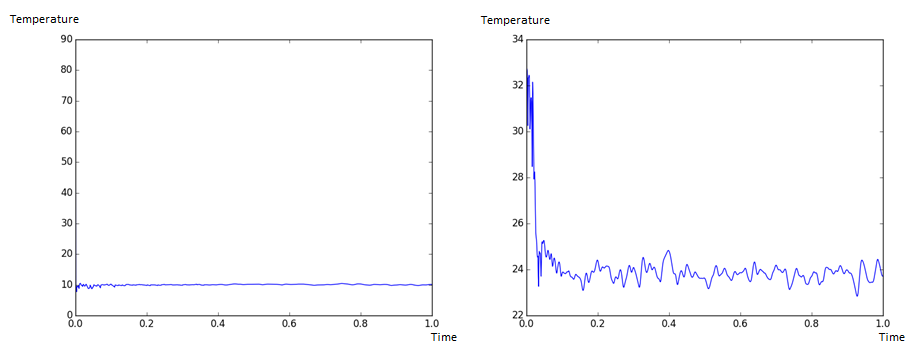
\includegraphics[width=140mm]{thermostat.PNG}
\caption{On the left the thermostat is disactivated. On the right the thermostat is activated until t=0.4}
\end{figure}

\section{Results}

Whereas most of the model is implemented in python, the nested loop necessary for the force calculation (the bottleneck of this algorithm) is written in Fortran for speed. The Fortran code is linked to python with the Fortran to Python Interface called f2py. The constants corresponding to physical constants or properties of Argon are taken equal to one. These include the mass of each particle, $\sigma$ and $\epsilon$ the two parameters in the Lennard-Jones potential and the Boltzmann constant. The number of particles is fixed to 864 at which the simulation takes a few seconds with a time step of 0.004.

\vspace{5mm}
A first result which proves the validity of our model is the conservation of the total energy. The potential energy is calculated as the sum of all the interaction potentials between two different particles, and the kinetic energy is taken to be the sum of the kinetic energy of each particle. The total energy is conserved with a standard deviation of  0.6 after the simulation converges as illustrated in fig 2 for T=0.1 

\begin{figure}[H]
\centering
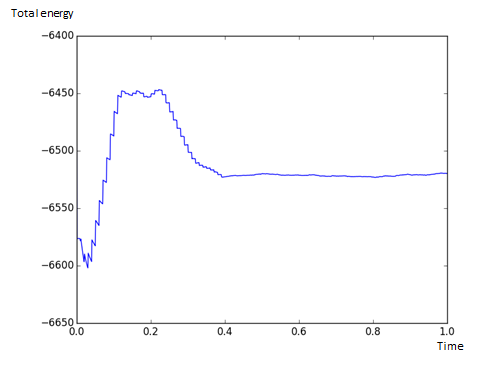
\includegraphics[width=80mm]{energy.png}
\caption{Time evolution of the total energy}
\end{figure}


The computation of the correlation function leads to knowledge about the state of the gas of Argon atoms. Indeed, depending on the initial temperature we get different results. In fig. 3 we see, from left to right the correlation function plotted for temperatures T = 0.1, 1, 10 corresponding to a solid, a liquid and a gas respectively. Also plotted are a 2 dimensional representation of the final positions of the particles.

\begin{figure}[H]
\centering
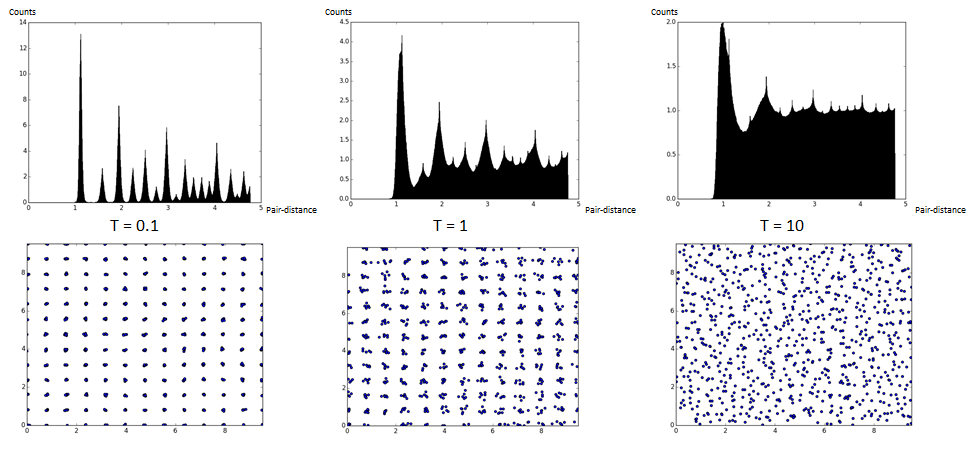
\includegraphics[width=140mm]{corr.PNG} % dummy filename
\caption{From left to right, the final positions an correlation functions for simulations with T = 0.1, 1 and 10} % Change N as necessary
\end{figure}

The pressure is calculated with the Virial equation corrected for the cut-off in the potential calculation [1]

\begin{equation}
\frac{p}{n{k_B}T} = 1 - \frac{1}{3N{k_B}T}[ \sum_{i}\sum_{j>i}{r_{ij}}\frac{\partial U(R)}{\partial r_{ij}} ]{_{cut-off}} - \frac{2\pi N}{3{k_B}TV}\int_{r_{cut-off}}^{\inf}r^3\frac{\partial U(r)}{\partial r}g(r)dr
\end{equation}

This allows the calculation of pressures for different temperatures as presented in the following. Note the convergence to an ideal gas state as the temperature increases (P/T converges to 1).

\begin{table}[h]
\centering
\begin{tabular}{|c|c|c|}
\hline

Temperature & Pressure & Variance \\ \hline
0.1         & 1.17     & 4.22e-07 \\ \hline
1           & 2.12     & 1.13-04  \\ \hline
10          & 11.15    & 8.32-03  \\ \hline
50          & 51.2     & 0.23     \\ \hline
\end{tabular}
\end{table}


\section{Conclusion}

We have achieved a realistic simulation of an Argon gas as shown by the energy conservation as well as the high temperature, ideal-gas limit. This allows us to explore properties such as the pressure in solid  liquid phase, phase transitions or the validity range of an ideal gas approximation. 

\vspace{5mm}

The simulation speed could be further improved by keeping track of the particles which are close to each other with a method such as the linked-cell method. This would allow simulations with more particles. We could also investigate other properties of the Argon gas such as the heat capacity.

\section{References}
[1] - "Computational Physics" J.M. Thijssen


\end{document}